\chapter{Results}

The aim of the methods described in this thesis is to provide tools to query the disequilibrium of sequence evolution. Described in this chapter is the characterisation of the developed methods. I present the application of the test of existence, and test of consistency to simulated data. Additionally, I present two new statistics for measuring the magnitude of disequilibrium. I evaluate these statistics on simulated data. I complement this with the results of the methods applied to empirical data where I expect disequilibrium to exist.

\section*{Developing and validating the methods}

A process of validation was applied to each method. A simple specification of methods is not enough, it is necessary to determine how it behaves and that it behaves in a way that matches up with the expectation when how the data is generated is known. There is an infinite number of way in which things can be out of equilibrium, but the number of ways in which they can be in equilibrium is a lot more restrictive. Since I am interested in departures from being in equilibrium, that’s the condition set that I have imposed in developing the methods. Below I describe the intent of a particular statistic, then describe the way in which it was developed.

\subsection*{The LRT for Existence with parametric bootstrapping provided a robust estimation of significance}

The test of existence seeks to determine whether the process is described significantly better by a non-stationary process. Formally, the test of existence is a LRT between the following hypotheses:\\ $\mathbf{H_0}$: the foreground evolved according to the \textbf{GNS}, the background according to BH. \\ $\mathbf{H_1}$: the foreground evolved according to the \textbf{GN}, the background according to BH.\\
Here I report the best methods of model fitting and the behaviour of the test in simulated data. 

It is important that the best possible methods of model fitting are chosen. A necessary precursor to any application of the test is to establish maximal fits of the models. Additionally, the process of fitting a model to an alignment is the most time-consuming method routinely used in my project. I have sought to identify the quickest possible method that yields a maximised likelihood. 

For this, I conducted an initialisation experiment that makes use of a property of nested models. For nested models, it is guaranteed that the likelihood for the alternate will be greater or equal to that for the null. General Time-Reversible (GTR) is the most general time-reversible process, and is required for my initialisation experiment. GTR is nested in GNS, which in turn is nested in GN. When a model is not maximally fit, the optimisation methods have failed to find the global maximum. Such is referred to as a local maximum, where they are higher points elsewhere but not nearby. In such cases, getting parameter estimates from a nested model fit to use as initial estimates may aid the optimisation in escaping a local maximum. I also wish to establish whether there is a speed gain in initialised model fits compared to uninitialised fits. Theoretically, if given starting values close to the optimal, this may reduce the time it takes to get there. 

For all synthetic data sets, I tested whether initialisation improved the model fitting process. The initialised method fit models in order of increasing generality (GTR, GNS, GN). Importantly, parameter estimates for each model were obtained from the previous model. The uninitialised method fit GNS and GN separately. The maximum likelihood estimates between uninitialised and initialised fits were compared for the models (e.g., uninitialised GN vs initialised GN). The time taken for each fitting process was recorded.  

The initialisation experiment revealed that there are no intrinsic problems with the fitting process for GN or GNS. A fit was considered non-maximal if the log-likelihood from the initialised method was higher than that of the uninitialised method. There were no occurrences of non-maximal fits for any of the synthetic alignments. Initialised fits which were faster than the corresponding uninitialised fits were rare, occurring at a rate of about ~1\%. These results suggest that the best method of fitting for both models is without initialisation.

To determine whether a given LRT statistic is significant requires establishing the appropriate null distribution. Statistical theory states that under certain conditions, the LRT statistic will be $\chi^2_{df}$ distributed with degrees freedom (df) equal to the difference in the number of free parameters between the models. In which case, one can obtain the p-values for a given LRT statistic simply from the analytical distribution. However, the behaviour of my test with real finite data is unknown. When considering the use of mixed discrete- and continuous-time Markov process is a deviation from convention, it is especially important to establish whether the test statistic is consistent with theoretical expectations. 

The distribution is closer to theoretical expectations for longer sequences, depicted in Figure \ref{fig:synthetic/lrt/197113-long_seq}. The figure shows data generated from the same high JSD, high entropy seed process, however, the results for all seeds were very similar, see appendix Figure \ref{fig:synthetic/lrt/all-seeds}. For alignments of length 300bp, shown in Figure \ref{fig:synthetic/lrt/197113-long_seq}a, the distribution of LRT statistic yields an excess of small p-values. Consequently, the data points of the Quantile-Quantile plot fall well below the diagonal line. Owing to increasing the power of the test, the distribution of p-values for longer alignments, illustrated in Figure \ref{fig:synthetic/lrt/197113-long_seq}b, is less skewed. Overall, the data points fall much closer to the diagonal line. It is worth noting that consistency with the theoretical distribution is most important for the smaller p-values. In Figure \ref{fig:synthetic/lrt/197113-long_seq}b, for quantiles corresponding to a significant test statistic (i.e. the bottom left corner where $p<0.05$), the distribution is very close to the theoretical distribution. This means that the chance of a false-positive is more or less in line with statistical expectations (5\%). Now, consider the distribution of p-values for $p>0.05$. Even though the distribution is not uniform, using the $\chi^{2}$ distribution, a non-significant result would still yield a non-significant p-value (true-negative). Thus, for some longer alignments, it may be suitable to assume the LRT statistics are $\chi^{2}$ distributed and in turn, obtain the p-value simply from analytical distribution. 

\begin{figure}[htbp]
\centering
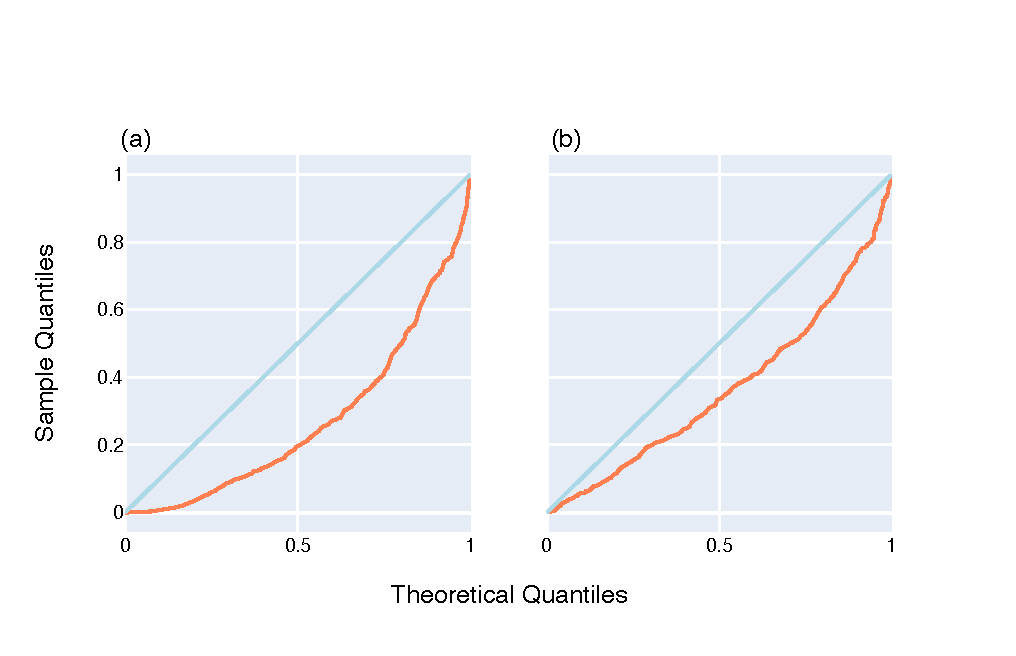
\includegraphics[width=\textwidth]{figures/plots/synthetic/lrt/197113_332182_17210-long_seq.pdf}
\caption[Increasing the length of the alignments gives a distribution of $\hat p-$ values closer, but not consistent with theoretical expectations]{\textbf{Increasing the length of the alignments gives a distribution of $\hat p-$ values closer, but not consistent with theoretical expectations.} The Quantile-Quantile (Q-Q) plots compare the $\hat p$-value distribution of the test for existence in stationary simulated data to the uniform distribution (pink line). Theoretical expectation is illustrated by the diagonal (blue line). Q-Q plot for \textbf{(a)} synthetic alignments of length $300$bp, \textbf{(b)}, synthetic alignments of length $30,000$bp. Each data set contains 1,000 synthetic stationary alignments. Both data sets shown are generated from the same high JSD, high entropy seed. The other seeds exhibited the same pattern, the result is shown in the appendix Figure \ref{fig:synthetic/lrt/all-seeds}.}
\label{fig:synthetic/lrt/197113-long_seq}
\end{figure}

The exploration with synthetic data clearly informs the application of my test. Firstly, results of the initialisation experiment show there is no intrinsic fitting problems. As such, model fitting in all cases will be done without initialised parameter estimates. The results in Figure \ref{fig:synthetic/lrt/197113-long_seq} demonstrate that I cannot assume the LRT statistic to be $\chi^{2}$ distributed. As conventional asymptotic approximations to the LRT distribution are shown not to apply, significance levels will need to be assessed via a parametric bootstrap. 

\subsection*{A transformed $\nabla$ statistic exhibited robust behaviour under the null}

The statistic $\nabla$ is a measure of the speed of convergence of the actual process to equilibrium. Consider a process operating on a single edge of a phylogenetic tree for a time interval of length $t$, for which the frequencies of nucleotides at the root is $\pi_0$ and the rate matrix on the edge is $Q$. The nucleotide distribution at $t$ is $\pi(t) = \pi_{0} \cdot e^{Qt}$. For a stationary process, this simplifies to $\pi(t) = \pi_{0}$. Under weak assumptions, a non-stationary process will converge to a stationary process, for which $\pi$ remains unchanged over time. Thus, I can describe the speed of this convergence with the rate of change of $\pi(t)$. In other words, the derivative of $\pi$ with respect to $t$,
\begin{equation}
\label{eq:dpi/dt}
\frac{\partial \pi}{\partial t}(t) = \pi_{0} \cdot Q \cdot e^{Qt}.
\end{equation}
To describe the magnitude of a vector in a single value, it is natural to take its length. Accordingly, the $\nabla$ statistic is defined as follows,
\begin{equation}
\label{eq:len-dpi/dt}
\nabla = ||\frac{\partial \pi}{\partial t}(t)|| =|| \pi_{0} \cdot Q \cdot e^{Qt}||.
\end{equation}
$\nabla$ is the magnitude of the rate of change of $\pi(t)$. For a stationary process, for which by definition $\pi$ does not change over time, $\nabla = 0$. For a non-stationary process, as the process approaches equilibrium, $\nabla$ will asymptote to $0$. Thus, a large $\nabla$ will likely correspond to a process that is far from equilibrium and a small $\nabla$ to a process that is close to equilibrium. The algorithm used to calculate $\nabla$ is presented in Algorithm \ref{alg:convergence}.

\begin{algorithm}[ht!]
\caption[Algorithm]{Calculating $\nabla$}
\label{alg:convergence}
\begin{minted}{python}
def convergence(pi_0, Q, t):

    pi_deriv = dot(pi_0, dot(Q, expm(Q * t)))
    conv = norm(pi_deriv)

    return conv
\end{minted}
\end{algorithm}


\begin{figure}[!ht]
\centering
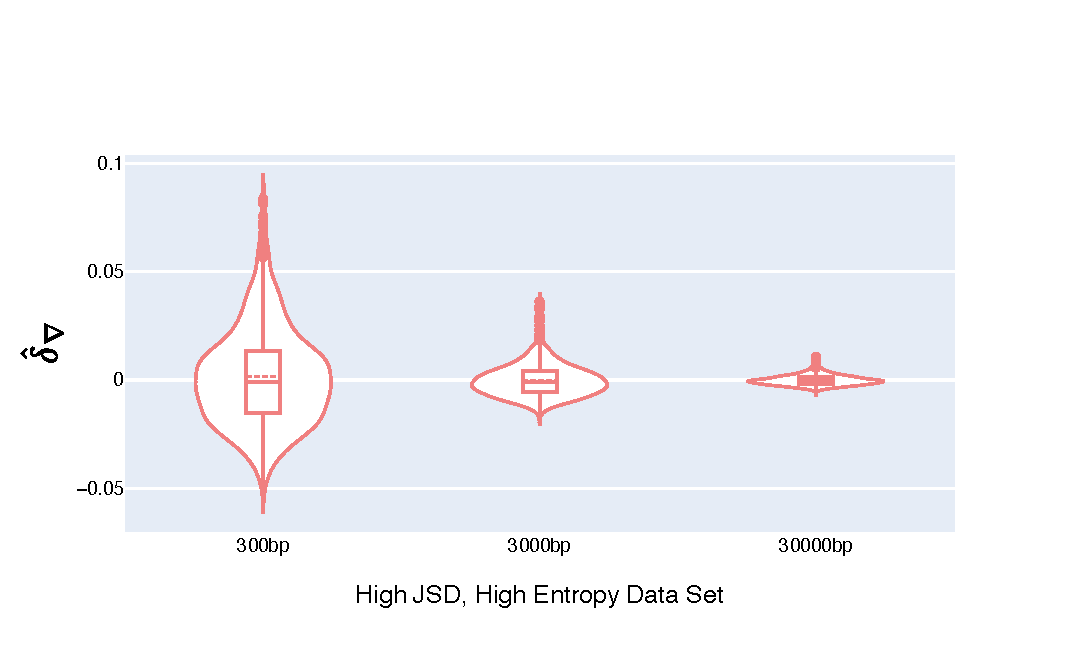
\includegraphics[width=\textwidth]{figures/plots/synthetic/d-conv/High JSD, High Entropy.pdf}
\caption{Centred on zero}
\label{fig:synthetic/d-conv/HighJSDHighEntropy}
\end{figure}




\subsection*{The $T_{50}$ statistic exhibited paradoxical properties that prevent interpretation}

A natural way to describe disequilibrium in a system is by its proximity to equilibrium. As previously stated, for a process in disequilibrium, as time goes to infinity, its nucleotide distribution will converge to $\pi_\infty$, its equilibrium distribution. This can be expressed mathematically as 
$$\pi_\infty = \lim_{t \to \infty}\pi \cdot e^{\mathbf{Q}t}.$$ 
This property manifests in other situations, for example the decay of a radioactive element. In those fields the problem of quantification is solved by expressing in terms of an arbitrarily chosen metric, half-life, the time taken until half of the element's original mass is left. ${T_{50}}$ is defined equivalently.

${T_{50}}$ is a measure of the distance to halfway to $\pi_\infty$, measured in terms of the expected number of substitutions. 

Put in that for a process in equilibrium it literally is zero because it is a good point.

\begin{algorithm}[ht!]
\caption[Algorithm]{Calculating $T_{50}$}
\label{alg:t50}
\begin{minted}{python}
class T50:
    def __init__(self, Q, pi_0, func=jsm):
        """
        func
            a callback function that takes two probability vectors
            and returns a "distance". Defaults to Jensen-Shannon metric.
        """
        self.Q = Q
        self.pi_0 = pi_0
        self.pi_inf = self.get_stat_pi()
        self.dist_halfway = func(self.pi_0, self.pi_inf) / 2
        self.tau = 1
        self.dist_func = func

    def get_stat_pi(self):
        return get_stat_pi_via_brute(expm(self.Q), self.pi_0)

    def estimate_t50(self):
        ens_curr = expected_number_subs(self.pi_0, self.Q, 1)
        self.tau = minimise(
            self,
            xinit=self.tau,
            bounds=([1], [1e10]),
            local=True,
            show_progress=False,
            tolerance=1e-8,
        )
        ens_50 = expected_number_subs(self.pi_0, self.Q, self.tau)
        return ens_50 - ens_curr

    def distance_from_pi_zero(self, pi):
        return self.dist_func(self.pi_0, pi)

    def __call__(self, tau):
        pi_tau = dot(self.pi_0, expm(self.Q * tau))
        dist1 = self.dist_func(self.pi_0, pi_tau)
        dist2 = self.dist_func(pi_tau, self.pi_inf)
        return abs(dist1 - dist2) ** 2
\end{minted}
\end{algorithm}


\subsection*{The tests of equivalence of process were consistent with asymptotic approximations}



\section*{Validation of method behaviour with empirical application}



\section*{Is the human genome at equilibrium?}